\documentclass[11pt,a4paper,titlepage,oneside]{report}

\usepackage[english]{babel}
\usepackage[utf8]{inputenc} % input encoding is UTF-8

\usepackage{graphicx}
\usepackage{tabularx}
\usepackage{subcaption}
\usepackage{apacite}
\usepackage{natbib}
\usepackage{color}
\usepackage[unicode,pdftex]{hyperref}
\usepackage{xcolor}

\hypersetup{
  colorlinks,
  linkcolor={red!50!black},
  citecolor={blue!50!black},
  urlcolor={blue!80!black}
}

\begin{document}

% Title page %%%%%%%%%%%%%%%%%%%%%%%%%%%%%%%%%%%%%%%%%%%%%%%%%%%%%%%%
\begin{titlepage}

\begin{figure}
\centering
\begin{subfigure}{.5\textwidth}
\centering

\includegraphics[width=0.8\textwidth]{img/logo_NTNU.png}\\
\end{subfigure}%
\begin{subfigure}{.5\textwidth}
\centering

\includegraphics[width=0.8\textwidth]{img/logo_SINTEF.jpg}
\end{subfigure}
\end{figure}

\begin{center}
{\LARGE \textbf{TDT4290 - Customer Driven Project}}
\vfill
{\Huge \textbf{Ocean forecast}}

\vspace{12pt}
{\LARGE \textbf{SINTEF}}

\vspace{30pt}
{\LARGE \textbf{Final report}}
\vfill
{\LARGE \textbf{Autumn 2014}}
\end{center}
\vfill
\begin{tabular*}{\textwidth}{@{\extracolsep{\fill}} l l}
\textbf{Group 6} & \textbf{Advisor} \\
Arve Nygård & Gleb Sizov \\
Anders Smedegaard Pedersen & \\
Emil Jakobus Schroeder & \\
Hans Kristian Henriksen & \\
Marco Radavelli & \\
Ondřej Hujňák & \\
Ruben Håskjold Fagerli & \\
\end{tabular*}

\end{titlepage}

% Empty page %%%%%%%%%%%%%%%%%%%%%%%%%%%%%%%%%%%%%%%%%%%%%%%%%%%%%%%%
\newpage
\thispagestyle{empty}
\mbox{}
\newpage

% Abstract %%%%%%%%%%%%%%%%%%%%%%%%%%%%%%%%%%%%%%%%%%%%%%%%%%%%%%%%%%
\begin{abstract}
Abstract
\end{abstract}

% Signatures %%%%%%%%%%%%%%%%%%%%%%%%%%%%%%%%%%%%%%%%%%%%%%%%%%%%%%%%
\thispagestyle{empty}
\begin{center}
{\large \textbf{Trondheim, \today}}\\
\vspace{2.5cm}
\begin{tabularx}{\textwidth}{@{\extracolsep{1cm}} X X }
\dotfill & \dotfill \\
~Arve Nygård & ~Anders Smedegaard Pedersen \\[1cm]
\dotfill & \dotfill \\
~Emil Jakobus Schroeder & ~Hans Kristian Henriksen \\[1cm]
\dotfill & \dotfill \\
~Marco Radavelli & ~Ondřej Hujňák \\[1cm]
\dotfill & \\
~Ruben Håskjold Fagerli & \\[1cm]
\end{tabularx}
\end{center}

% Table of contents %%%%%%%%%%%%%%%%%%%%%%%%%%%%%%%%%%%%%%%%%%%%%%%%%
\tableofcontents
\addtocontents{toc}{\protect\thispagestyle{empty}}

% List of figures %%%%%%%%%%%%%%%%%%%%%%%%%%%%%%%%%%%%%%%%%%%%%%%%%%%
\listoffigures
\addtocontents{lof}{\protect\thispagestyle{empty}}

% List of tables %%%%%%%%%%%%%%%%%%%%%%%%%%%%%%%%%%%%%%%%%%%%%%%%%%%%
\listoftables
\addtocontents{lot}{\protect\thispagestyle{empty}}

\pagenumbering{arabic}
\setcounter{page}{0}

% Main body %%%%%%%%%%%%%%%%%%%%%%%%%%%%%%%%%%%%%%%%%%%%%%%%%%%%%%%%%
%%%%%%%%%%%%%%%%%%%%%%%%%%%%%%%%%%%%%%%%%%%%%%%%%%%%%%%%%%%%%%%%%%%%%

\chapter{Introduction}
\section{TDT 4290 - Customer driven project}
The task is set forth in the subject TDT 4290 - Customer driven project at the Norwegian university of science and technology. The goal of the course is 
\begin{quote}
(...)to give the students a practical experience of carrying out all the phases of a typical customer guided IS/IT-project. \citep{TDT4290:Intro}
\end{quote}
The subject divides the students into random groups, and assigns each group an assignment. The assignments are real problems that businesses needs solved. 

Although the assignment is to follow the entire process of an IT-project, the focus is on the earlier phases of a project. Thus, an important part of the assignment is the work leading up to the implementation phase. There is obviously also an important focus on the implementation itself. Maintenance is however left out of the scope of the projects.

\section{Customer}
The customer is SINTEF Fisheries and Aquaculture (SINTEF Fiskeri og havbruk AS). 
SINTEF was founded in 1950 and it is nowadays organized into 8 divisions. The division of Fisheries and Aquaculture was founded in 1999 and represents technological expertise and industry knowledge in the utilization of renewable marine resources. Under the vision \"Technology for a better society\" it works for a knowledge-based bio marine industry. Its goal is to meet market demands for technological research and development on renewable marine resources.

\section{Ocean currents}
About currents, why they are important, who is interested etc.

\section{Assignment and scope}
The client, SINTEF Fisheries and Aquaculture, has given us the project labeled ”Ocean Forecast”. The task is to improve the actual system of storing and retrieving data for the monitored and predicted parameters of ocean.

\chapter{Planning}
This section will give an overview of our plans for the project. It will include time estimation, group organization, risk management and quality assurance.

The name of the project and the scope of the assignment has already been introduced in the previous section.
\section{Project stakeholders}
The stakeholders of this project are the following:
\begin{description}
\item[Project owner (customer)] SINTEF Fisheries and Aquaculture
\item[Supervisor (from NTNU)] Gleb Sizov
\item[Examiner] External examiner, nominated by the direction of the course TDT4290 - Customer Driven Project
\item[Team members (students)] 
\end{description}

\section{Background for the project: software system development}
The customer owns a working solution, running on its own servers, for the delivery and analysis of marine tracked and predicted data, in form of maps with overlays and charts.
The background for this project is to optimize the actual, slow and memory-consuming solution, with a new one, and/or creating new front-end application using those data, to cover more use-cases.

\section{Measurement of project effects}
Some predefined criterias must be met in order to consider out project a successful one. Our product must be working according to the requirements and pass all tests in order to be a success. All requirements prioritized high and medium must be fulfilled. Requirements that have low priority are optional, but should be implemented if there is sufficient time.
In our case, quite open goals were requested by the customer, and no precisely quantifiable measurements were defined.
If working on improving the actual solution the measurements should be:
\begin{itemize}
\item The time it takes to visualize data for the end user should be “reasonably low” even with slow internet connection (like from Chile) or from a mobile device
\item The same displayed features as the actual working system are still available
\end{itemize}
If working on new use cases, the measurements should be:
\begin{itemize}
\item The same displayed features as the actual working system are still available
\item New features (such as mobile app and new charts) are added in order to cover more use-cases 
\end{itemize}
In both cases, an open source based solution is considered to be better than a commercial one.

\section{General terms}
The choice implementation language, platform and tools to use are up to us. The requirement is that the solution should run on a server.
There are non-functional requirements, in terms of improving performance and storage consumption, that should be accomplished.

\section{Planned workload}
Group members will aim to work 24-25h on average per week, for a total amount of 12 weeks. Group members can distribute the workload among days according to their lecture timetibles, as long as deadlines (including sprints deadlines) are met.
Our group consists of 7 people, so that the weekly average amount of workload is globally around 168-175h, for a total of 2016-2100 h.

\section{Schedule of results}
We are using a Scrum-like project management framework, and working prototypes are expected to be produced at the end of each speint. Requirements have been prioritized by the customer with numbers from 1 to 100. The requirements for our project are inevitably overlapping, and almost all the requirements must be accomplished in order to produced a working solution, to satisfy the basic project goal requested by the customer.

\section{Concrete project work plan}
This section describes the specific layout of the project. This project follows the Scrum methodology with some variants introduced, as discussed in the appendix. The first five weeks were spent planning, pre-studies (which included a preliminary implementation of the critical part of the system), and writing the requirement specification. As a common practice, the project was divided into sprints. We decided to make each sprint lasting one week. At the end of the last sprint all the requirements should be accomplished.
\subsection{Phases}
We decide to the Scrum methodology, so that Scrum sprints characterize the phases of the project.
The following are the phases that can be distinguished in the project:
\begin{itemize}
\item Initiation phase (pre-planning)
\item Project Planning
\item Project Prestudy Sprint (Sprint 0)

\item Sprint 1
\item Pre-delivery of report (17th October)

\item Sprint 2
\item Sprint 3
\item Sprint 4

\item Demo Planning
\item Project Delivery and Demonstration
\end{itemize}

\subsection{Activities}
\begin{description}
\item[Pre-planning] During the pre-planning activity, the group members know each other and understand the task. There are also the first meetings with the customer and with the avisor.
\item[Pre-study and planning] The pre-study and planning activity is the stage where the actual work on the project begins. We explpore solutions and we determine which technologies will be used and how the product will be realized.
\item[Documentation] The documentation activity represents time spent documenting the work effort, including implementation, research etc., and administrative tasks like status reports and documents for the meetings.
\item[Coordination] The coordination activity is accomplished throughout the project, and consists of activities to coordinate the work, such as meetings, internal emails, calls and messages.
\item[Implementation] The implementation activity consists of the implementation of the system. This includes the programming of both the back end and the front end part.
\item[Testing] The testing activity represents time spent testing the system. This includes integration testing, unit testing, functional testing and scenario-driven testing.
\item[Presentation] The presentation activity is the final presentation of the system and the delivery of the report.
\end{description}

\subsection{Milestones}
We defined some milestones in order not to create delays in the progress of the project.
There are some milestones defined by the course structure, and we decided to add some more "internal" project milestones in order to avoid delays.
The following are the defined milestones:
\begin{description}
\item[October 6th] Pre-study phase to be completed
\item[October 17th] Pre-delivery of report (defined by the course coordinators)
\item[November 17th] Project report to be completed
\item[November 20th] Final presentation day (defined by the course coordinators)
\end{description}

\subsection{Person-hours per activity and phase + lectures + project management}
In this projects there have been a number of guest lectures, and we have made sure that every lecture were attended by at least one member in the team.

\section{Project Organization}
\subsection{Organizational diagram of how the group is organized}

\begin{figure}[h]
\begin{center}
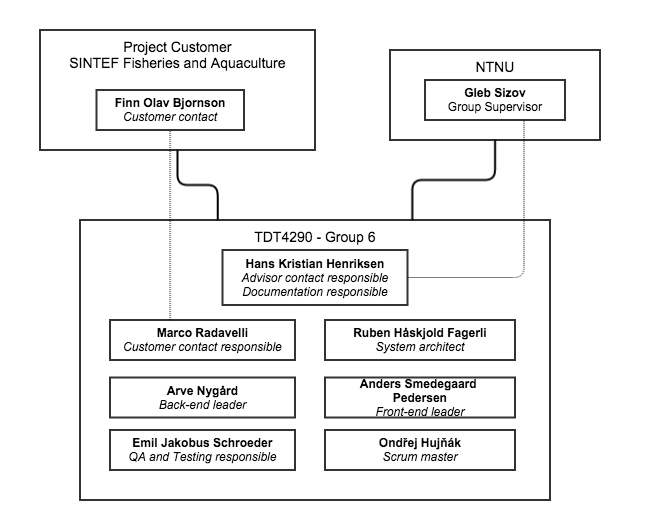
\includegraphics[height=260px,width=328px]{img/tdt4290_group_6_organizational_structure.png}
\caption{Organizational diagram. The arrows indicate the bi-directional communication. The dotted arrows denotes the preferred way of communication between components. Note that the layout is not hierarchical and it is arranged this way only to better fit on the printed page.}
\label{fig:organizational-structure}
\end{center}
\end{figure}

\subsection{Roles and corresponding responsibilities}
We defined and diveded roles and responsibilities among group members. We agreed the distribution of the responsibilities by the voluntary choice of the role for each component of the group, and internal unanimous agreement.
We conveyed the following roles:
\begin{description}
\item[Scrum master] His task is to make sure that we meet our goals, he is the first person who talks to the customer and to the advisor in the meetings, make sure that the groups meetings have a structure and that they finish on time. According to the scrum methodology, the scrum master also has to supervide the scrum pocess (control that is respected), remove eventual impediments to the team's work, protect team from distracting influences, and make sure that the team is on-task.
\emph{Role assigned to: \textbf{Ondřej Hujňák}}
\item[Customer contact] His task is to arrange customer meeting, forward customer emails to the group if needed, and ensure that all the needed communication with the customer is done.
\emph{Role assigned to: \textbf{Marco Radavelli}}
\item[QA and testing responsible] Ensure that the implementation fulfills the requirements, design test plan, define and ensure that the Quality Assurance standard is followed during the project.
\emph{Role assigned to: \textbf{Emil Jakobus Schroeder}}
\item[Documentation responsible] Supervise the structure and the content of all the documents (report, status reports, agenda and minutes of meetings, pre-study report). Main responsible to take notes during meetings. 
\emph{Role assigned to: \textbf{Hans Kristian Henriksen}}
\item[Advisor contact] Arrange advisor meetings, send documents (status report, agenda and minutes of last meeting) to the advisor before each meeting.
\emph{Role assigned to: \textbf{Hans Kristian Henriksen}}
\item[Front-end leader] Supervise the front-end architecture and implementation, and coordinate the front-end developer team
\emph{Role assigned to: \textbf{Anders Smedegaard Pedersen}}
\item[Back-end leader] Supervises the back-end architecture and implementation, and coordinate the back-end developer team
\emph{Role assigned to: \textbf{Arve Nygård}}
\item[System architect] Make sure that there is consistency between requirements, design and implementation, and that the design is feasible and reasonable.
\emph{Role assigned to: \textbf{Ruben Håskjold Fagerli}}
\end{description}

\subsection{Weekly schedule}
We decided to adopt a scrum-like model of software development, with internal group meetings twice a week, weekly meetings with the advisor and meeting with the customer when needed (typically every other week). The schedule is defined as follows:
\begin{itemize}
\item Mondays 2-3 pm - Advisor meeting
\item Mondays 3-4pm - Team meeting
\item Thursdays 12-2pm - Team meeting
\end{itemize}
For weeks 37 and 38 the advisor meeting will be Thursday 4pm.

We decided to use the academic quarter for internal meetings, but to start the meeting at the time conveyed sharp for advisor meetings.

\chapter{Tools and technology}
\section{Documents}

  \subsection{\LaTeX}
  \LaTeX~is a typesetting system and document markup language that became standard for scientific documents. It is easily expandable by thousands of different packages and can handle all aspects of scientific papers.

  We have chosen to use \LaTeX~for our report for two main reasons - \LaTeX~sources are easily readible and, because they are simple text files, they can be easily versioned by various version control systems. Second reason was focus on content, not on form. In \LaTeX~sources there is only very little information about exact view of the page. \LaTeX~itself during compile time chooses the best position of elements so it complies with all typographic norms.

  We have created a template in our shared space together with a bibliography file. Everyone could then write his sections in an environment that suited him the best while the current state of the report was always available to all members.

  \subsection{Google Docs}
  Google Docs \footnote{\url{https://docs.google.com}} is a web based office suite including a text editor, a spreadsheet program and a presentation program. All files created in these programs can easily be shared with colaborators. By sharing files the colaborators get access to view and edit the files. Editing and commenting on other's work. We decided to use Google Docs for all documents that did not require the advanced typesetting of \LaTeX~so we had a common platform for such documents.

\section{Project management}
  \subsection{Trello}
Trello is a web-based collaborative project management tool originally made by Fog Creek Software (New York, USA) \footnote{\url{http://www.fogcreek.com/}}. 
It's based on the Kanban method which has first implemented by Toyotain 1953 to be used in car production. It has since been modified to be used in several different industries. 
David J. Anderson formulated a model based on Kanban for knowlegde based work, specifically software development, where the team work incrementally pulling work from a queue \citep{da2004}. 
This work queue in represented by a card for each task wich is located in a "to-do" area on a board. Task may then be moved to a bin called for example "in progress" to indicate that the task is beeing work on. Finally, when the task is complete, the cars can be moved to a "done" bin. In Trello this is implemented by elements you can drag and drop between bins. As an administrator you have the possibility to define both bins and boards which makes Trello a very versatile tool.  
Trello is a freemium webservice which means that it is free to use but additional support and features can be accessed if you pay a fee. As we only needed the standard functions and thus used the free version.
  \subsection{Slack}
Slack is a webbased team communication tool founded by Stewart Butterfield. It offers text chat in different channels and integration with a number of different popular services used by development teams \footnote{\url{https://slack.com/integrations}}. This was useful to us since we needed to share information that might be more relevant to specific team members and also to have a single means of communication. Using Slack's integration with Trello and Github we would get notified when there where changes on these platforms aswell. Slack's posibillity to share files, or link to files on Google Documents also came in handy.

\section{Version control}
  \subsection{Git}
  Git is a distributed version control system developed in 2005 by Linus Torvalds and Linux development community \citep{ProGit}. Git was made to be small, fast and easy to use especially for code management as it's main purpose was versioning of Linux kernel source code. Nowdays is Git one of the most used versioning controls systems in software development thanks to it's open linence and powerfull features.

  We have chosen Git because some members already know it and are able to work efficiently with it. Another advantage is easy branching and distributed architecture that allows you to work offline. 
  
  We have created an organization on GitHub\footnote{\url{https://github.com}} with multiple repositories for different separate parts of our work - reports, server sources, client sources. We have chosen GitHub because it is well known git hosting server that offers advanced features and stability. Moreover some members already had accounts on GitHub and were familiar with interface, which shortened time needed to setup a working environment.

\section{Programming languages}
  \subsection{Java}
  Java is a popular programming language developed by a team led by James Gosling at Sun Microsystems in 1991. It's full-featured , general purpose language capable of developing robust mission-critical applications \citep{liang}. This and the fact that everybody in the group had at least basic knowlegde of Java led to the dessicion that we would use Java for our back-end application.  
  \subsection{JavaScript}
  As stated by Davis Flanagan i JavaScript: the definitive guide "Javascript is part of the triad of technologies that all Web developers must learn". He continues to note that JavaScript specifies the behaviour of the web page \citep{fd11}. Along with specification of HTML5 and ECMAscript 6 (the standard name of JavaScript) the posibilities of what you can achieve with JavaScript has greatly improved. Since our assignment was to create a web based solution it seamed natural to use JavaScript as part of the solution. This was further supported by the excistence of open source libraries designed to make interactive maps which was relevant for our assginment.

\section{IDEs}

\chapter{Pre study}
In this chapter, we present the findings of the pre study. The pre study document was made as a separate document that was meant to be delivered to the customer independently of this report. Therefore, there are overlapping sections with the full report. These sections will not be given in this chapter, but are instead presented in their respective chapters of the full report. 

\section{Background}
To get an understanding of the customers needs, as well as studying different solutions, a pre study is conducted. From the course compendium:
\begin{quote}
The preliminary studies are vital for the group to obtain a good understanding of the total problem.
Here, you will have to describe the problem at hand. You should describe the current system and the
planned solutions (...).
\cite{TDT4290:Intro}
\end{quote}

\section{Use cases}
SINTEF has put forth a series of situations were their system is used by the fishery industry. 
\begin{itemize}
\item \textbf{Planning of new fish farm sites} \\
When choosing a new site for a fish farm, it is important to be aware of historical information on currents, temperature and salinity. Placing a new site in an area that has high currents might make construction and other operations difficult.
\item \textbf{Planning the removal of lice in a fish farm} \\
In the event that lice has to be removed from the fish in the farm, there are two procedures that are used. In the first scenario, a tanker vessel will pump the fish from the farm into a holding room. Here, the fish is treated with chemicals before being pumped back to the farm. The second method brings in crane boats, that hoist the farm, thus shrinking the volume the fish has available. A canvas is then used to surround the fish, and the chemicals are added directly. 

Both these operations require calm currents, as to ensure that any support vessels are able to stay in position during the operation. Having access to the latest current predictions is vital in the planning of this type of operation.
\item \textbf{Planning feeding of fish in fish farms} \\
The fish in a farm is kept in close confinement. When the fish is fed, their activity rises significantly, consuming larger amounts of oxygen than usual. Given the right combination of temperature and currents, this could lead to oxygen levels dropping to dangerously low levels. Being able to plan feeding in accordance with forecasts for temperature and currents minimizes the risk of harm to the fish.
\end{itemize}

\section{Current situation at SINTEF}
In this chapter we will explore the solution SINTEF is currently using, and the challenges and limitations it poses. After looking into this, we will describe the evaluation criteria that will be used to assess the alternative solutions the group has found. 
\subsection{Current system}
\begin{figure}[h]
\begin{center}
\fbox{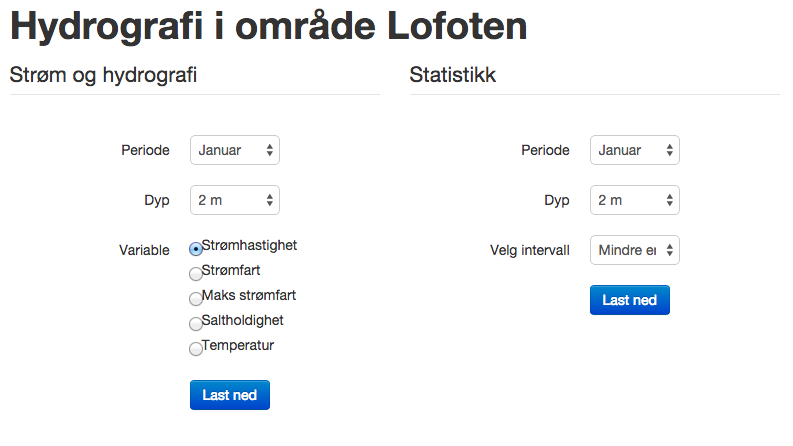
\includegraphics[height=223px,width=396px]{img/region_interface_sinmod.png}}
\caption{The main interface for a region in SinMod}
\label{fig:sinmod-region-main-interface}
\end{center}
\end{figure}

The current system deployed at SINTEF serves their clients by providing access to a collection of more than 100 000 pre generated PDF files. These files contain information on currents, salinity, and temperature. The user may choose what information he\footnote{"He" should be read as "he or she" throughout this report} wants by selecting parameters in the drop down menus, see figure \ref{fig:sinmod-region-main-interface}.

\begin{figure}[h]
\begin{center}
\fbox{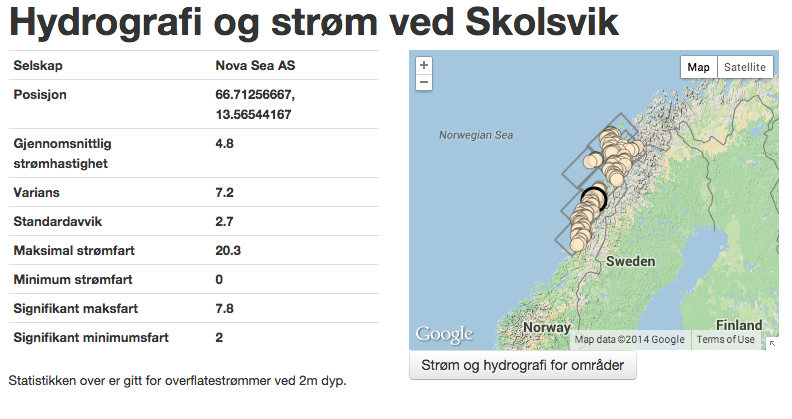
\includegraphics[height=223px,width=396px]{img/site_key_data.png}}
\caption{The key data a user is presented with when selecting a specific site}
\label{fig:sinmod-site-key-data}
\end{center}
\end{figure}

If the user chooses a specific site from the map or location drop down, he will be presented with key data for this area. This includes statistical information such as maximum current speed, average current speed and so forth, as well as geographical position, as given in figure \ref{fig:sinmod-site-key-data}.


\begin{figure}[h]
\begin{center}
\fbox{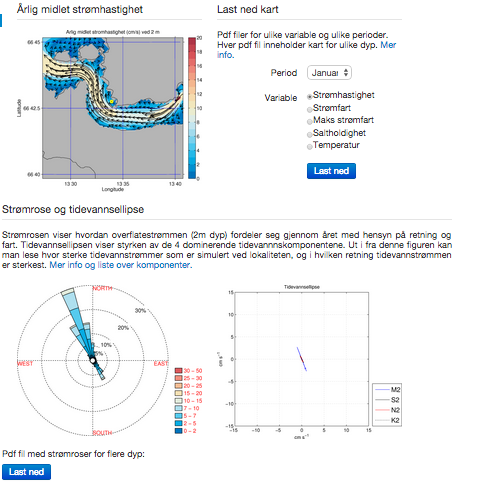
\includegraphics[height=300px,width=300px]{img/site_graphs.png}}
\caption{Some of the graphs presented to the user when selecting a specific site}
\label{fig:sinmod-site-graphs}
\end{center}
\end{figure}

The system will also present a set of pre defined graphs, including current roses, tidal ellipsis and vertical profiles. The graphs are given for standard attributes (e.g depth 2 meters), and for some of them, there is an option of downloading a PDF containing graphs for other values of the given attributes. An example is shown in figure \ref{fig:sinmod-site-graphs}


\subsection{Challenges}
As the PDFs are pre generated, there is a clear limitation to what information the user may request. If a user wants to know, for example, the connection between salinity and current speed at a given location, the user must download two different PDFs and manually compare these. 

The graphs given for a specific location are only given for limited values of the critical attributes. If we look at the current rose, it is presented for a depth of 2 meters. If the user is really interested in the current rose for 10 meters, he has to download the PDF containing all possible current roses. 

The same is true for the maps that can be generated for a specific site. The user may choose period (a single month may be selected), and one of the five variables. This gives the user a PDF with one map for each depth that can be calculated. 

For a user who knows what data is interesting, this is a complicated and data heavy way of delivering information. The PDFs seems to range in size from 125kB to around 3MB, depending on what information is requested. The region maps are the absolute largest in file size, ranging from 1 to 3MB, while the files containing the current roses are quite small, in the 100-200kB range. 

On a computer with broadband connection, the size of the files is not very problematic. For these users, the biggest challenge is the fact that the user can not specify what kind of data they want plotted, and have to look through quite a lot of pages to get the information needed. For a user on a low bandwidth connection and/or on a mobile device, the size of the files is a more pressing problem. On an EDGE connection the theoretical best download time for a 3MB file is 62,5 seconds at 384kbit/s \cite{3gpp.com}.

\subsection{Evaluation criteria}
SINTEFs main goal with this project is to be able to rid themselves of the PDF store, and generate the information on demand. This will make for a much more flexible system, where it will be possible to add new graphs and functionality quickly. For the customers, it will make it possible to request more customised graphs and plots.

SINTEF has presented the group with several goals they wish the new system to fulfil:

\begin{itemize}
\item The system should generate the graphs and maps directly from the NetCDF files on user request.
\item The user should be able to select several variables for one plot.
\item The system should be usable on low bandwidth connections.
\item The system should be usable on mobile devices.
\item The system should be easy to expand with new functionality.
\end{itemize} 

With these goals in mind, the group started looking into different technologies that could be used to make such a system.

%%%
\section{Other production solutions}
The group has used the first part of the project investigating what solutions would best suit SINTEFs needs. In the chapter we present the different solutions we have found, along with an assessment on how each solution is rated in accordance to the evaluation criteria. 

%Existing tech - Italian solution
\subsection{Adriatic Forecasting System}
\emph{Link: \url{http://oceanlab.cmcc.it/afs/}} \\%make sure to use //
  The solution, by the Operational Oceanography Group Italy and cmcc Ocean-Lab, can display temperature, salinity, currents, sea surface height, wind stress and heat flux. It allows the user to choose date, region and depth as search filters, and uses PNG overlays on a Google map. The PNGs are retrieved from cmcc's own server.
  Although it graphically looks quite nice, it can be seen that some tiles are not precisely overlapping. In addition, sometimes it is needed to refresh the page because the application doesn't load properly. PNG layers are displayed without a specific JS library, and the JS code is quite complex compared to other existing solutions using libraries. Therefore this solution is not well re-usable.
\\ \emph{Overall rating: \textbf{Ok}}

\subsection{Danish Centre of Ocean and Ice}
  \emph{Link: \url{http://http://ocean.dmi.dk/anim/index.uk.php }} \\%make sure to use //
    The solution by the Danish Center of Ocean and Ice can display temperature, salinity and current, which are the most important factors of the SINTEF simulation. This said, it lacks the ability to choose depth and specify a date interval. The data is shown as static PNGs, thus the map is not interactive. There is, on the other hand, a possibility to choose different geographical areas with the highest level of detail around Denmark. This is on the same level as SINTEF's existing solution.
  \\ \emph{Overall rating: \textbf{Bad}}

  \subsection{Fisheries and Oceans Canada}
  \emph{Link: \url{http://www.tides.gc.ca/eng}} \\%make sure to use //
    The solution of the Canadian government resembles the Danish one. It is possible to choose a geographical area on a static map. By choosing an area you get the opportunity to choose a smaller, more specific area. The big difference is that all data is presented as text in tables, thus making it less convenient and intuitive to use.
  \\ \emph{Overall rating: \textbf{Bad}}

  \subsection{Ocean viewer}
  \emph{Link: \url{http://www.oceanviewer.org}} \\%make sure to use /
    Ocean Viewer is a pilot project of the Marine Environmental Observation Prediction and Response Network (MEOPAR) of Canada. It gathers data from different sources and displays it as PNGs overlayed on a map. You can select different geographical areas on a customized Google Map and different data from a menu (temperature, salinity and others). Like the Danish solution the PNGs can be shown in sequence to show changes over time.
  \\ \emph{Overall rating: \textbf{Ok}}

  \subsection{Sea temperatures and Currents - Bureau of Meteorology}
  \emph{Link: \url{http://www.bom.gov.au/oceanography/forecasts/}} \\%make sure to use //
    The Australian Bureau of Meteorology has a solution that is very similar to the other national agencies. You can choose a geographical area on a static map. Here as well, the data is visualized with images overlayed on a static map, with the possibility to loop through the images to show changes in the data over time.
  \\ \emph{Overall rating: \textbf{Ok}}
  
  \subsection{yr.no Map Service}
  \emph{Link: \url{http://yr.no/kart}} \\%make sure to use //
This solution presents the user with a conventional map interface. On the sides and top there are menus for selecting which variable and timestep should be displayed. The user is only allowed to select a timestep about 8 days from the current time. Interesting variables include sea temperature, salinity and sea currents, each has it’s own . There is no way to select depth, and all data seems to be for the surface values. The chosen variable is added as an overlay of PNG tiles using OpenLayers. The tiles are fetched using WMS from a norwegian meteorological service server. On the map there are several measurement stations displayed, that give information when clicked. In addition, clicking anywhere on the map displays several plots predicting the next two days of weather for that spot.
  \\ \emph{Overall rating: \textbf{Ok}}

\section{Back-end}

\subsection{GeoServer}
Does not support NetCDF natively. There exist a community plugin that enables you to read from NetCDF files, but the support seems very shifty. GeoServer does not seem to have support for more than one file and metadata appears difficult to extract. Due to this factors, the system was deemed to not to meet the needed criteria.

\subsection{THREDDS}
\begin{quote}
The THREDDS\footnote{\textbf{Th}ematic \textbf{R}ealtime \textbf{E}nvironmental \textbf{D}istributed \textbf{D}ata \textbf{S}ervices} Data Server (TDS) is a web server that provides metadata and data access for scientific datasets, using OPeNDAP, OGC WMS and WCS, HTTP, and other remote data access protocols. \cite{TDS:Web}
\end{quote}

  Except supporting multiple data access protocols, TDS is able to virtually aggregate multiple NetCDF files to one dataset that can be used for queries, such as selecting a region and sending it's data in specified format. Dataset configurations are done via NcML\footnote{\textbf{N}et\textbf{C}DF \textbf{M}arkup \textbf{L}anguage}, which is a dialect of XML.

  Although TDS seems to support everything that is needed for this project, it's installation, and especially configuration for agreggation and special needs, is not trivial. Moreover there are doubts about speed and dealing with serving a range containing large quantified points. One advantage is that SINTEF currently have a TDS running and configured, so we won't need to configure it from scratch, and SINTEF employees probably have experience and knowledge about setting it up, something which the group lacks.

  \subsection{Custom solution}
  An alternative is to write a custom back-end from scratch.
  Advantages of this are:
  \begin{itemize}
  \item Easy deployment - written as a single service that you just launch.
  \item Load balancing - Easily scale outwards: The servers can be put behind a load balancer. 
  \item Speed - No overhead for unused features.
  \item Code clarity - No overhead for unused features.
  \end{itemize}
  A skeleton for the whole server is in place. Below is a list of features that the group feels are within reach in the project period. 
  \begin{itemize}
  \item Indexing and file selection.
  \item Projection (Mapping between latitude/longitude and file indices)
  \item Filtering (Reducing the result set before reading the file)
  \item Output
  \item Rendering to image
  \item Rendering to GeoJSON
  \end{itemize}

  Performance seems to be very good at the current level of implementation. The only major potential bottleneck the group sees is reading files from a hard-drive. (All testing has been done on SSDs). This bottleneck will however be independent of backend solution.
  
  \subsection{MapTiler}
  \emph{Link: \url{http://www.maptiler.org/}} \\%make sure to use //
    MapTiler is an application for online map puplishing. It makes it possible to create tiles that can be overlayed over other maps like Google Maps, Open Street Map and others. It's written in C/C++ and claims to be a lot faster than other existing solutions. A draw back seems to be that it's made for overlaying a pre generated directory of images rather than dynamic data like the ocean forecast data.
  \\ \emph{Overall rating: \textbf{Ok}}
  
    \subsection{ncWMS}
  \emph{Link: \url{http://www.resc.rdg.ac.uk/trac/ncWMS/}} \\%make sure to use //
    ncWMS is an open source, free to use, java server application. It was created to support interactive browsing of gridded four-dimensional netCDF data over the web. Clients will send request containing the wanted coordinates (latitudes, longitudes, depth and time), what variable is to be displayed, projection, format and size the response should be. ncWMS, which has been configured to read from datasets (for example sets of netCDF files or a THREDDS server), responds to a request with an image of the desired type. ncWMS adheres to the WMS specification (WMS 1.3.0 and 1.1.1 are supported).
    \paragraph{Configuration}
    ncWMS is mainly configured through a web interface, where you can add datasets and change server settings. A dataset can be: a single netCDF file, an OPeNDAP endpoint (a service provided by THREDDS), a NcML file or a glob aggregation (using wildcard characters like ). It is possible to configure which variables of a dataset to expose and how. Each dataset can also be set to automatically refresh at certain intervals. The server can be set to cache data, to reduce cpu load at the expense of memory and disk space.
    \paragraph{Aggregation}
    The glob aggregation or NcML work well with files that cover the same area, but contain different timesteps. To handle different areas and different resolutions it may be possible to use THREDDS/OPenDAP or NcML.
    \paragraph{Perfomance}
    Testing both local and publicly available ncWMS servers the performance seems good. When using the godiva2 browser based client or sending individual requests the server mostly responds quickly, with some idiopathic exceptions. Transmitting the map data to the client as png images should be a bandwidth-efficient way to do it, as well as moving the computation load away from the client. When starting the server application or adding a dataset, the server needs some time to load some information from the datasets. This only takes a few seconds, even for a few hundred GB of local netCDF files.
    \paragraph{Summary}
    ncWMS does a lot of what we need the back-end of our solution to do. It handles the extraction, downsampling and projection of the data, creating an image ready to be used in a map widget or on it’s own. It can only handle requests for a few kinds of plots. It is open source, and is free to use under a modified BSD license. To serve all the plots and data required it would need modification.
  \\ \emph{Overall rating: \textbf{Good}}

%%%
\section{Transmission Protocols}
  There are several standardized protocols to present map data from the server to the client in order to dinamically display layers on a map.
  In particular, two main kind of representations can be distinguished, and sometimes they're both supported by a single standard:
  \begin{description}
    \item[Vector based layers] Data is sent from the server to the client in a textual format, such as GeoJson
    \item[Image based layers] Data is sent from the server to the client as images, such as Jpeg, png and gif
  \end{description}

  The Open Geospatial Consortium (OGC) became involved in developing standards for web mapping after a paper was published in 1997 by Allan Doyle, outlining a \"WWW Mapping Framework\". The oldest and most popular standard for web mapping is WMS. However, the properties of this standard proved to be difficult to implement for situations where short response times were important. For most WMS services it is not uncommon to require 1 or more CPU seconds to produce a response. For massive parallel use cases, such a CPU-intensive service is not practical. To overcome the CPU intensive on-the-fly rendering problem, application developers started using pre-rendered map tiles. Several open and proprietary schemes were invented to organize and address these map tiles. 
  In order to reduce the performace problems of WMS, new standards have been defined:
  \begin{itemize}
    \item TMS
    \item WMS-c
    \item WMTS
  \end{itemize}
  
  \subsection{WMS}
    Web Map Service (WMS) is a standard protocol for serving georeferenced map images over the Internet that are generated by a map server using data from a GIS database. The specification was developed and first published by the Open Geospatial Consortium in 1999.
    A WMS server usually serves the map in a bitmap format, e.g. PNG, GIF or JPEG. In addition, vector graphics can be included: such as points, lines, curves and text, expressed in SVG or WebCGM format.
    The WMS standard allows flexibility in the client request enabling clients to obtain exactly the final image they want. A WMS client can request that the server creates a map by overlaying an arbitrary number of the map layers offered by the server, over an arbitrary geographic bound, with an arbitrary background color at an arbitrary scale, in any supported coordinate reference system.

  \subsection{TMS}
    Tile Map Service or TMS, is a specification for storing and retrieving cartographic data, developed by the Open Source Geospatial Foundation. The TMS protocol fills a gap between the very simple standard used by OpenStreetMap and the complexity of the WMS standard, providing simple urls to tiles while also supporting alternate spatial referencing system.
    TMS is most widely supported by web mapping clients and servers, and it is served as the basis for WMTS (the OpenGIS Web Map Tile Service OGC standard).

  \subsection{WMS-c}
    The WMS Tiling Client Recommendation, or WMS-C for short, is a recommendation set forth by OSGeo for making tiled requests using WMS. It is just a recommendation on using WMS properly in order to improve performance by caching data.
    This recommendation relies on two basic concepts to support this purpose: First, cachability of map imagery can be improved by using image tiles of fixed width and height, referenced to some fixed geographic grid at fixed scales. A valid tile request is one that conforms to the specification of fixed image parameters and geographic grid(s) for a given layer. By analogy, an invalid tile request is one that does not.
    Second, caching of HTTP GET requests is further made possible by constraining the URL parameters used in the request. This recommendation identifies the WMS GetMap parameters minimally needed for a client to request a valid tile.

  \subsection{WMTS}
    Web Map Tile Service (WMTS) is a standard protocol for serving pre-rendered georeferenced map tiles over the Internet. The specification was developed and first published by the Open Geospatial Consortium in 2010
    WMTS builds on efforts to develop scalable, high performance services for web based distribution of cartographic maps. To define this standard, similar initiatives were also considered, such as Google maps and NASA OnEarth. WMTS includes both resource (RESTful approach) and procedure oriented architectural styles (KVP and SOAP encoding) in an effort to harmonize this interface standard with the OSGeo specification.
    WMTS complements earlier efforts to develop services for the web based distribution of cartographic maps. The OGC WMTS provides a complementary approach to the OGC Web Map Service (WMS) for tiling maps. WMS focuses on rendering custom maps and is an ideal solution for dynamic data or custom styled maps. WMTS trades the flexibility of custom map rendering for the scalability possible by serving of static data (base maps) where the bounding box and scales have been constrained to discrete tiles. The fixed set of tiles allows for the implementation of a WMTS service using a web server that simply returns existing files. The fixed set of tiles also enables the use of standard network mechanisms for scalability such as distributed cache systems.

  \subsection{Summary}
    WMS-C is the best supported and most mature protocol, but it's a bit of a kludge overlayed on top of WMS to support tiles and it incurs some extra overhead from having to use world coordinate bounding boxes rather than tile coordinates.
    TMS is fairly mature, and is specifically designed for tiles, but is not an official OGC spec.
    WMTS is an OGC spec that is meant to replace TMS and WMS-C. It works purely in tile coordinates like TMS (although it computes them differently) but has some additional capabilities that weren't in TMS, like GetFeatureInfo. It's comparatively recent, but it is becoming more and more used, even if its implementations are less mature. It is also supported by OpenLayers.

%%%
\section{Frontend solutions}
  A central part of the product requirement is to display simulated data in a dynamic manner. There exists solutions to do just that, and javascript libraries than makes it relatively easy to create at front end solution of our own. In this section we will discuss and compare the most relevant of these in the context of our assignment and the product requirements. 
  \subsection{Custom made solution}
    A custom made solution has the general advantage that we can built it to specification and thus make sure it meets the requirements without having to deal with other peoples code base. Trying to customize an existing solution might be as much work as building something from the bottom. In the following paragraphs we will review and rate technologies we found relevant for building a custom front end.
    \subsubsection{LeafletJS}
    \begin{tabular}{|p{4cm}|p{8cm}|}
      \hline
      Home page: & \url{http://www.leafletjs.com} \\
      \hline
      Service functionality: & Creating mobile-friendly interactive maps. \\
      \hline
    \end{tabular}
    
    \paragraph{Introduction} \indent
    LeafletJS ("Leaflet" for the rest of the section) is an open source javascript library for creating mobile-friendly interactive maps. It's licensed under the \href{'https://github.com/Leaflet/Leaflet/blob/master/LICENSE'}{2-clause BSD License}, which makes it free to use in commercial applications as long as a credit is added somewhere in the user interface.
    Even though Leaflet is free to use it is dependent on a third party to provide the map tiles. These may not be free to use.

    \paragraph{Features}
    Leaflet has the features you'd expect from a modern interactive map. This includes paning with inertia, zooming and the ability to add markers. It also supports double-tap and pinch to zoom for IOS and Android on mobile phones. Furthermore all the five biggest web browsers are supported, including graceful fallback for old versions.
    
    The most powerful feature of Leaflet is the ability to add layers. The different supported layers are:

    \begin{itemize}
      \item Tile layers
      \item Marker layers
      \item Pop-ups
      \item Vector layers
      \item GeoJSON layers
      \item image overlays
      \item WMS layers
      \item Layer groups
    \end{itemize}

    For our purposes the ability to get map tiles from different sources may be very interesting. This gives us the ability to for example show both nautical maps and regular land maps at the convenience of the user. At zoom levels covering large geographical areas it will probably be most ideal to show the relevant simulated data as overlayed PNGs. This is easily achieved with image overlays in Leaflet. If we want to show very detailed data when zoomed further in, we might be able to use vector layers to visualize the data. It is also possible to use a GeoJSON layer to convert data formatted as GeoJSON to vectors.
    It is also possible to use Web Map Service (WMS) to overlay, for example, metrological data on a map. Eventhough this is a format that is used by large organizations like the National Oceanic and Atsmopheric Administration (\url{noaa.gov}) we have been advised against using this format due to it's negative effect on the speed and responsiveness experienced by the end-user. \footnote{Iván Sánchez Ortega, How to Build Slow Maps - Trondheim, September 24, 2014}
    Furthermore Leaflet can be extended with plugins. These can relatively easily be written in Javascript or an existing plugin can be downloaded and used. A relevant plugin to our needs could for example be heatmap.js (\url{http://www.patrick-wied.at/static/heatmapjs/}).

    \paragraph{Summary}
    Leaflet is very suitable for our needs in respect to creating an interactive map overlayed with visualizations of relevant data created by the SINTEF ocean forecast simulations. It's lightweight(33 kilobytes), made to be compatible with mobile phones and very flexible in possibilities to display data on maps. It's also well documented.

  \subsubsection{OpenLayers}
   \begin{tabular}{|p{4cm}|p{8cm}|}
     \hline
     Home page: & \url{http://openlayers.org/} \\
     \hline
     Service functionality: & A high-performance, feature-packed library for all your mapping needs. \\
     \hline
   \end{tabular}
   \paragraph{Introduction} \indent
   OpenLayers is an open source (provided under the \href{'https://tldrlegal.com/license/bsd-2-clause-license-(freebsd)'}{2-clause BSD License}) JavaScript library for displaying map data in web browsers. It provides an API for building rich web-based geographic applications similar to Google Maps and Bing Maps. The library was originally based on the Prototype JavaScript Framework. Since November 2007 OpenLayers is an Open Source Geospatial Foundation project.
   The current stable version, OpenLayers 3.0, has been released August 29, 2014.
   \paragraph{Features}
   OpenLayers provides support to the following functionalities:
   \begin{description}
     \item[Tile layers] It pulls tiles from OSM, Bing, MapBox, Stamen, MapQuest, and any other XYZ source you can find. OGC mapping services and untiled layers also supported.
     \item[Vector layers] Renders vector data from GeoJSON, TopoJSON, KML, GML, and a growing number of other formats.
     \item[Fast \& Mobile Ready] Mobile support is out of the box, and it is possible to build lightweight custom profiles with just the needed components.
     \item[Cutting Edge \& Easy to Customize] Map rendering leverages WebGL, Canvas 2D, and HTML5. Map styling is controlled with straight-forward CSS.
   \end{description}
   \paragraph{Initial load time}
   The initial load time of the map is ok on a PC. The total loading time of the example (html with map and WMS tiles) took around 4 seconds. The size of the Javascript library (ol.js) is 129 KB, and the first time (without any sort of browser caching) it was fetched in 473 ms.
   \\ \emph{Score: \textbf{Med}}
   \paragraph{Responsiveness}
   It's quite fast when pan, but not so fast when zooming in (438 ms + 2.43 s for DNS lookup of the WMS server in the example) or out (around 400 ms was logged, on average, as the time to get tiles from the server, because there is no need of DNS lookup, but the overall perceived time is around 1s).
   \\ \emph{Score: \textbf{Med}}
   \paragraph{Detail and dynamism}
   The detail of the image is defined by PNG provided by the WMS server. Vector layers are also well drawn. Tile layers are updated on zooming.
   \\ \emph{Score: \textbf{High}}
   \paragraph{Ease of use}
   It is quite easy to implement. The code needed is low, and it is easily convertable into Leaflet format. There are a lot of provided working examples, but it is not well documented yet for the version 3.0 (that has been released very recently: at the end of August 2014). Anyway, the detailed API documentation is provided.
   \\ \emph{Score: \textbf{Med}}
   \paragraph{Summary}
   It is a library used in a lot of applications, dynamic, with a lot of features. On the contrary, it is less lightweight than LeafletJS, not so well documented and not always so fast as experienced by the user, especially in zooming.
   \\ \emph{Overall rating: \textbf{Good}}
  
  \subsubsection{Wind map}
  \emph{Link: \url{http://hint.fm/wind/}} \\%make sure to use //
    Wind map is a personal art project that gets surface wind data from the American government agency National Digital Forecast Database and displays it as moving curved lines on a map. This makes for a very intuivive visualization of the data that give a good general picture of the actual real-world situation. It's zoomable and can pan. By clicking on a specific point on the map you get the wind speed and coordinates of the point. A draw back might be the use on moblie devices which may be suboptimal.
  \\ \emph{Overall rating: \textbf{Good}}

  \subsubsection{Comparison of Leaflet and OpenLayers}
    For the purpose of creating an interactive map we've boiled it down to either using LeafletJS or OpenLayers. As the description of each of the individual libraries above shows, the two are have many of the same capabilities. Both gives us the posibility to overlay visulizations of data in different ways. An reason for choosing Leaflet is the extensive documentation of the current version, a point where OpenLayers are lacking at the moment. Despite this OpenLayers support of WMTS and WMSC is such a strong argument in it's favor that we jugde it as the best fit for our purposes.
    
  \subsection{Godiva2}
     \begin{tabular}{|p{4cm}|p{8cm}|}
     \hline
     Example page: & \url{http://behemoth.nerc-essc.ac.uk/ncWMS/godiva2.html} \\
     \hline
     Service functionality: & A browser client made to browse data served by a ncWMS server. \\
     \hline
   \end{tabular}
   
  \paragraph{Introduction}
  Godiva2 was created as a companion for ncWMS, to display the pngs served by ncWMS as tiles in a map interface. It is a fairly simple html page using JavaScript. \\
   It presents the user with a pannable, zoomable map interface of the earth. Variables (for example ocean temperature) can be selected from a menu. An overlay is added to the map, and the map zooms and pans to show the relevant area. The user can select the date, time of day and depth, updating the map immediately. Clicking on the map brings up a context menu, where a vertical profile plot can be created for that spot. Selecting a tool in the map interface, the user can draw a line on the map, and a plot is created showing the value of the selected variable along that line. There is a menu to select a different WMS, changing the background map and projection of any overlays. The site allows the user to grab a permalink of the current state of the map.

	\paragraph{Load time}
	Before selecting a variable, only a list of available variables and the background map are fetched. Testing Godiva2 on a local ncWMS server the initial load time is low. Tests using publicly available datasets vary, but some have low load time, indicating that the slower ones might just have less available resources.
   \\ \emph{Score: \textbf{Good}}
	
	\paragraph{Responsiveness}
	The responsiveness of panning and zooming the map, as well as changing the desired depth and timestep varies quite a bit. This is true both for local and remote datasets.
   \\ \emph{Score: \textbf{Medium}}
	
	\paragraph{Detail and dynamism}
	Every bit of detail available in the dataset is shown, as required by the level of zoom.
   \\ \emph{Score: \textbf{High}}
	
	\paragraph{Ease of Use}
	The menus for changing variable, depth and timestep are all intuitive and easy to use. The map interface follows the conventions for zooming and panning with the mouse.
   \\ \emph{Score: \textbf{High}}
	
	\paragraph{Summary}
	This is a product made to browse 4 dimensional geospatial data like the ones we want to present. The look and feel is slightly outdated, but the functionality it has works well. It is open source. It and the third party libraries are licensed under free software licenses. It (and the ncWMS server) would need to be modified in order to display all the data and charts found in the current solution.
   \\ \emph{Overall rating: \textbf{Good}}
	

\section{Recommendation}
Based on the study of possible solutions in the previous chapter, the group has made the following recommendation to the customer.

\subsection{Front-end}
As the group has looked into the situation at SINTEF, as well as other solutions in production, the conclusion is rather clear. SINTEF requires a very specific front end, with custom graphs, and the ability to add more functionality at a later stage. As far as existing solutions go, only the Godiva2 system has been close to performing the necessary tasks to serve SINTEFs needs. This system is however not very easy to adapt, and the group is of the opinion that changing this system to fit custom needs may be too much work to justify.

With this in mind, the group feels that the only realistic solution for the front-end is to develop a custom system from scratch.

\subsection{Back-end}
For the back-end, the group is divided in its recommendation. From our investigation into different technologies, it seems like THREDDS is a solution that is generally implemented for working with NetCDF files. Advantages of using this is that there exists documentation, maintenance, and updates. The group has had trouble configuring THREDDS, and has also gotten the impression that SINTEF is not perfectly satisfied with its performance. 

The group feels confident that a custom back-end prototype can be made, and that it will be able to meet the requirements. This will give the customer more flexibility in functionality and expandability, but will obviously not be as complete or well supported as THREDDS.

The group asks SINTEF to make a decision for a back-end solution based on the information in this report.

\subsection{Different paths}
As SINTEF is given a choice for how to proceed, the group sees two paths forward in the project:
\begin{enumerate}
\item THREDDS back-end: Given that SINTEF chooses to use a THREDDS back-end, the group asks SINTEF to provide a configured THREDDS server. The group will focus their work on the front-end, and attempt to make a prototype that replicates most functionality from todays site.
\item Custom back-end: Given that SINTEF chooses a custom back-end, the team will split into two groups, and attempt to make a prototype back-end, as well as a prototype front-end. In this scenario, both the front- and back-end will have limited capabilities, but will demonstrate what is possible with a fully custom solution.
\end{enumerate}


\chapter{Requirements}

\chapter {Pre-sprint work}

\chapter{Sprint 1}

\chapter{Sprint 2}

\chapter{Sprint 3}

\chapter{Sprint 4}

\chapter{Final solution}

\chapter{Evaluation}


% Sources cited in the document
% uncomment when there are some citations, uncomment bibtex in Makefile
%\bibliographystyle{plain}
\bibliographystyle{apacite}
\chapter{Bibliography}
\begin{flushleft}
	\bibliography{report}
\end{flushleft}

% Appendixes
\appendix

\end{document}
